\chapter{System Evaluation}\label{chap:eval}
One of the aims stated for this study, as listed in the Chapter~\ref{sec:Introduction}, was to write a Python application with scalability in mind. Therefore, this chapter is devoted to presenting a thousand-feet view of the application so that the implementation described in former chapters could be taken as only one of the many possibilities to realise the intended system characteristics as well as functionality. The second section of the chapter presents a discussion of SmartNotes application metrics gathered using benchmarking tools such as \texttt{autobench} or \texttt{siege} and statistics from the Google App Engine dashboard. The present chapter, together with Chaper~\ref{cha:conclusions}, also summarises the results of the subject of this study. 
 
\section{Presentation of the final result}\label{sec:result}
Apart from a client-server architecture whose segments were presented in Figure~\ref{fig:smartnotes_components}, SmartNotes has the features of flexibility, scalability and security described in Section~\ref{sec:gae}. The web interface of the application is a simple, internationalized one that provides general information about the project and allows the iterated users access its functionality. Currently, the latter involves merely creating a SmatNotes account by using the Google Account as described in Section~\ref{subsec:ismartnotes_activation} and later receiving an activation key, the process being straightforward as presented in Figure~\ref{fig:sn_web_interface}. Finally, the users pass the activation code to the iSmartNotes application in order to take the advantage of synchronization feature allowing the users, as described in Section~\ref{sec:functionality_descr}, to work on their notes and perform synchronization whenever they may wish. The main iSmartNotes window is presented in Figure~\ref{fig:ismartnotes_window}; specifically, it has a simple text area where notes can be edited, and a \texttt{Sync} button that, depending on network connectivity, will perform synchronization on the local machine or additionally using the SmartNotes network infrastructure. This basic attempt realises the functionality, excluding sharing and grouping notes which are extensions to the present functionality and will be added to the SmartNotes application beyond the focus and implementation completed in this study. It can be clearly noted that the tool cannot compete with such applications like the ones introduced in Section~\ref{sec:popular_apps}. Yet, the related work was used as a inspiration for creating a scalable foundation that could be later become more complex by adding additional functionality, hence making the gathered experience further expanded and rendering SmartNotes more attractive to users. Finally, the SmartNotes blog, feedback form and hosting the source code on a well known Open Source service does not only point to gather users’ attention, but also to find developers who find the idea interesting and collaborate on it. 
 
Technologies chosen here provide a well documented and truly active environment with a relatively low access barrier allowing direct involvement in a short time. Some of the chosen solutions, like Django or Mercurial, could become substituted with their equivalents among different language environments or using the Java language as a universal binding for the tools\footnote{Java programming language is wide know for its dynamic curve of development and impressing thread management. These features are few on the list of characteristics motivating the existence of such projects as JRuby, Jython or Quercus which are Java implementations of respectively Ruby, Python and PHP languages. That way, different runtimes can be used in one common environment, taking advantage of all of Java’s features.}.       
\begin{figure}[ht]
  \begin{center}
    \subfigure[\textbf{SmartNotes homepage with basic information and authentication}.]{\label{fig:sm_main}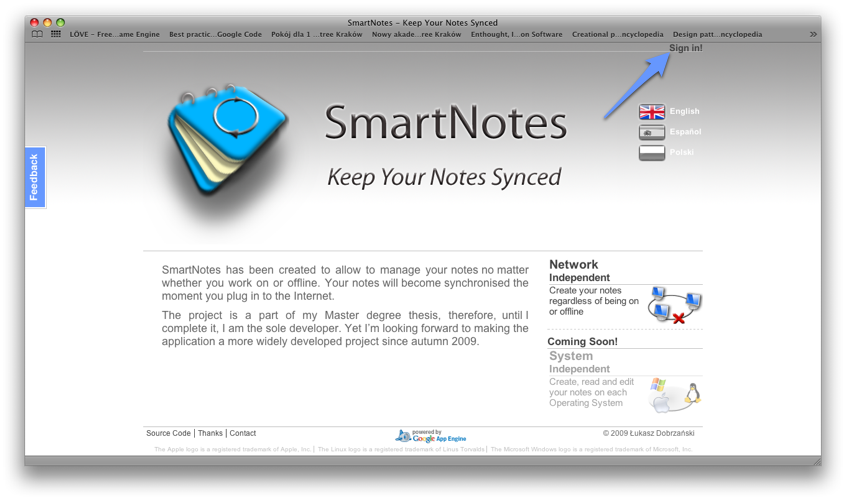
\includegraphics[scale=0.5]{img/SNmain_page.png}}
    \subfigure[\textbf{Authentication using the Google account}.]{\label{fig:sm_signin}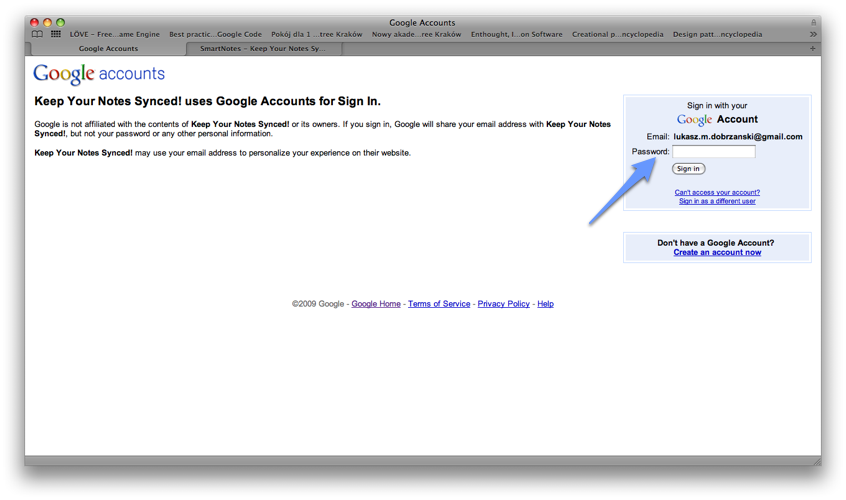
\includegraphics[scale=0.24]{img/SN_signin.png}}
    \subfigure[\textbf{Obtaining the SmartNotes activation key}.]{\label{fig:sm_getSNkey}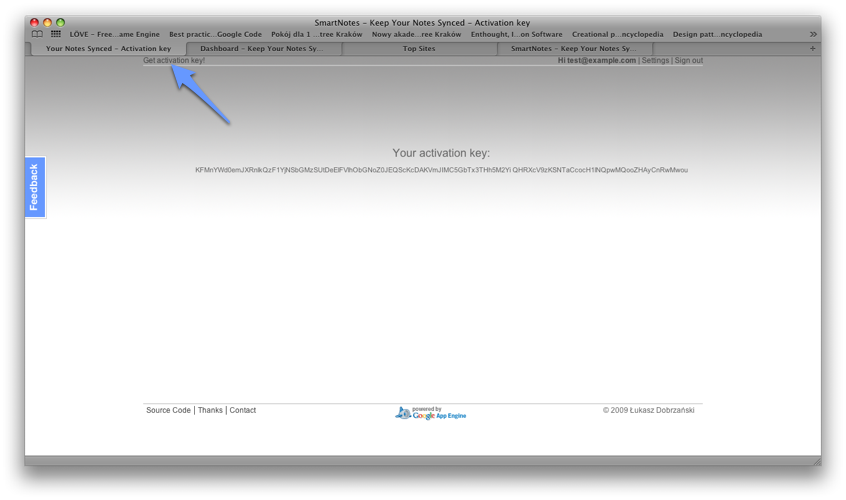
\includegraphics[scale=0.24]{img/SNget_activation_key.png}}
  \end{center}
  \caption{The view on the public web-based SmartNotes interface with basic information regarding the project and authentication.}
  \label{fig:sn_web_interface}
\end{figure}
That direction of development appears to be gathering popularity and is worth attention. However, the chosen set of components including:
 \begin{itemize}
        \item{Google App Engine -- as a platform providing scalable infrastructure and additional useful API's for mailing, imaging or remote task queues.}
        \item{Django famework -- one of Python web frameworks which attracts more and more developers trough its clean architecture, out-of-the-box usability and strong community.}
        \item{Mercurial -- pure Python version control system with a well-designed support for HTTP protocol and a zero cost of administration.}
 \end{itemize} 
is remains significantly powerful, allowing to carry out the desired functionality with easiness for further development, an aspect that should be always recalled during any design process or when choosing between concurrent solutions. That, combined with system streamlining for concrete use cases, determines why the entire system concept is highly desirable when building scalable systems.
        
\begin{figure}[ht]
\begin{center}
\includegraphics[scale=0.5]{img/SN_ismartnotes_window.pdf}
\caption{The view on the iSmartNotes application window.}
\label{fig:ismartnotes_window}
\end{center}
\end{figure}
 
\section{Performance tests}\label{sec:performance}
This subsection presents a graphical illustration of some chosen performance metrics of SmartNotes application running on Google App Engine. Taking into account the concurrency factor of incoming requests and the rate in which the  connection rate becomes increased the factors that will be analysed include:
\begin{itemize}
	\item{Minimum reply rate - }
	\item{Average reply rate - }
	\item{Maximum reply rate -}
	\item{X}
\end{itemize}
The tests were performed for main SmartNotes web page by using tools like \texttt{httperf} and \texttt{autobench} and collected data allowed to make graphs shown in Figure
\begin{figure}[ht]
  \begin{center}
    \subfigure[\textbf{X}.]{\label{fig:sm_main}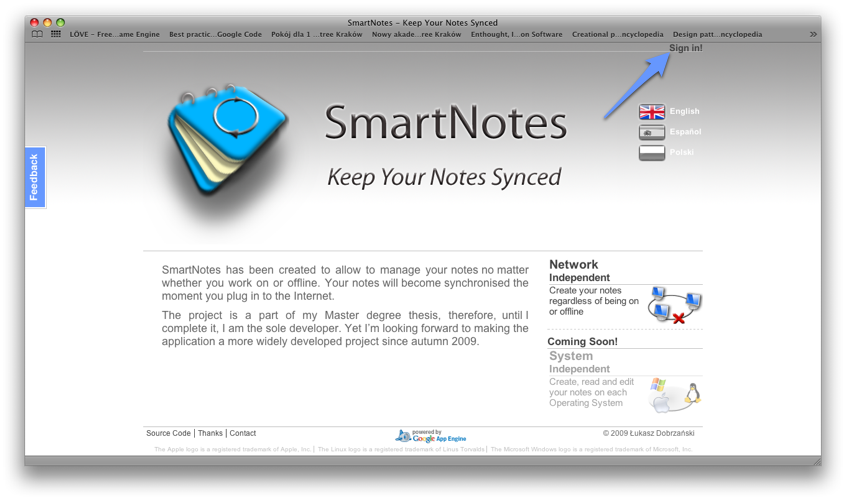
\includegraphics[scale=0.5]{img/SNmain_page.png}}
    \subfigure[\textbf{Y}.]{\label{fig:sm_signin}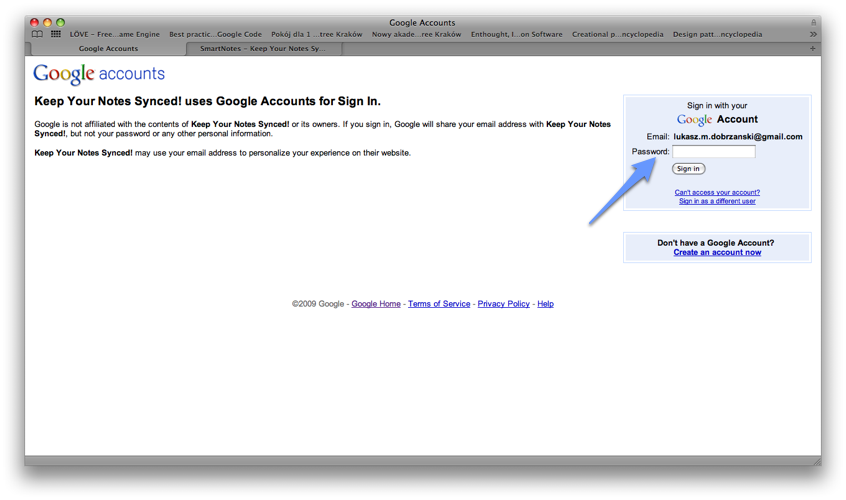
\includegraphics[scale=0.24]{img/SN_signin.png}}
    \subfigure[\textbf{Z}.]{\label{fig:sm_getSNkey}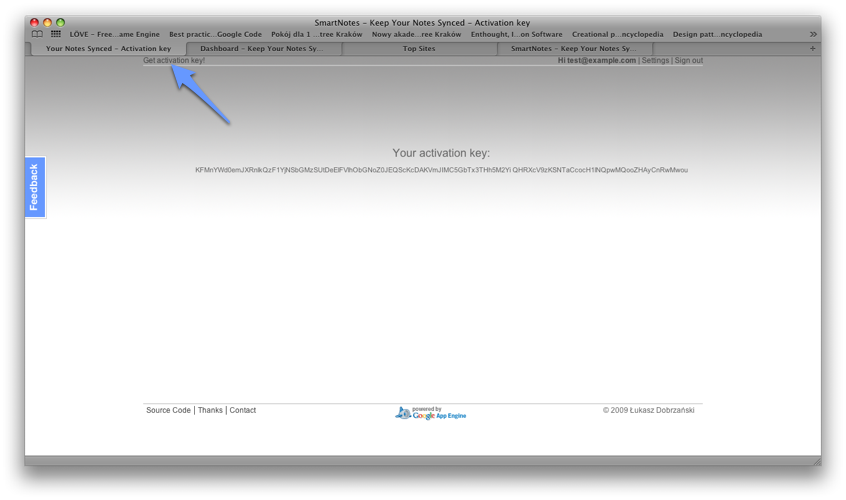
\includegraphics[scale=0.24]{img/SNget_activation_key.png}}
  \end{center}
  \caption{SmartNotes performence statistics.}
  \label{fig:sn_web_interface}
\end{figure}


   